%%%%%%%%%%%%%%%%%%%%%%%%%%%%%%%%%%%%%%%%%
% Stylish Article
% LaTeX Template
% Version 2.1 (1/10/15)
%
% This template has been downloaded from:
% http://www.LaTeXTemplates.com
%
% Original author:
% Mathias Legrand (legrand.mathias@gmail.com) 
% With extensive modifications by:
% Vel (vel@latextemplates.com)
%
% License:
% CC BY-NC-SA 3.0 (http://creativecommons.org/licenses/by-nc-sa/3.0/)
%
%%%%%%%%%%%%%%%%%%%%%%%%%%%%%%%%%%%%%%%%%

%----------------------------------------------------------------------------------------
%	PACKAGES AND OTHER DOCUMENT CONFIGURATIONS
%----------------------------------------------------------------------------------------

\documentclass[fleqn,10pt]{SelfArx} % Document font size and equations flushed left

\usepackage[spanish,english]{babel} % Specify a different language here - english by default
\PassOptionsToPackage{spanish}{babel}

\usepackage{svg}
\usepackage{booktabs}
\usepackage{listings}
\lstset{
  basicstyle=\ttfamily, %\fontsize{7}{11}
  stringstyle=\ttfamily,
  columns=fullflexible,
  frame=single,
  breaklines=true,
  postbreak=\mbox{\textcolor{red}{$\hookrightarrow$}\space}
}
\renewcommand{\lstlistingname}{Listado}

% Default fixed font does not support bold face
\DeclareFixedFont{\ttb}{T1}{txtt}{bx}{n}{9} % for bold
\DeclareFixedFont{\ttm}{T1}{txtt}{m}{n}{9}  % for normal

% Custom colors
\usepackage{color}
\definecolor{deepblue}{rgb}{0,0,0.5}
\definecolor{deepred}{rgb}{0.6,0,0}
\definecolor{deepgreen}{rgb}{0,0.5,0}

% Python style for highlighting
\newcommand\pythonstyle{\lstset{
language=Python,
basicstyle=\ttm,
otherkeywords={self},             % Add keywords here
keywordstyle=\ttb\color{deepblue},
emph={MyClass,__init__},          % Custom highlighting
emphstyle=\ttb\color{deepred},    % Custom highlighting style
stringstyle=\color{deepgreen},
frame=tb,                         % Any extra options here
showstringspaces=false            % 
}}

% Python environment
\lstnewenvironment{python}[1][]
{
\pythonstyle
\lstset{#1}
}
{}

% Python for inline
\newcommand\pythoninline[1]{{\pythonstyle\lstinline!#1!}}

\usepackage[utf8]{inputenc}
\usepackage{textcomp}
\usepackage[edges]{forest}

%----------------------------------------------------------------------------------------
%	COLUMNS
%----------------------------------------------------------------------------------------

\setlength{\columnsep}{0.55cm} % Distance between the two columns of text
\setlength{\fboxrule}{0.75pt} % Width of the border around the abstract

%----------------------------------------------------------------------------------------
%	COLORS
%----------------------------------------------------------------------------------------

\definecolor{color1}{RGB}{0,0,90} % Color of the article title and sections
\definecolor{color2}{RGB}{0,20,20} % Color of the boxes behind the abstract and headings

%----------------------------------------------------------------------------------------
%	HYPERLINKS
%----------------------------------------------------------------------------------------

\usepackage{hyperref} % Required for hyperlinks
\hypersetup{hidelinks,colorlinks,breaklinks=true,urlcolor=color2,citecolor=color1,linkcolor=color1,bookmarksopen=false,pdftitle={Title},pdfauthor={Author}}

%----------------------------------------------------------------------------------------
%	ARTICLE INFORMATION
%----------------------------------------------------------------------------------------

\JournalInfo{AGETIC Investiga, Vol. I, No. 1, 2018} % Journal information
\Archive{Agencia de Gobierno Electrónico y Tecnologías de la Información y Comunicación} % Additional notes (e.g. copyright, DOI, review/research article)

\PaperTitle{Desarrollo de comunicación HRP con antenas RFID Clou/Hopeland} % Article title

\Authors{Arturo Hernandez Calleja\textsuperscript{1}*} % Authors , James Smith\textsuperscript{2}
\affiliation{\textsuperscript{1}\textit{Profesional de Investigación, Area de Investigación, Unidad de Innovación Investigación y Desarrollo, AGETIC}} % Author affiliation
%\affiliation{\textsuperscript{2}\textit{Carrera de Ingeniería Electrónica, Facultad de Ingeniería, UMSA}} % Author affiliation
\affiliation{*\textbf{Contacto}: ahernandez@agetic.gob.bo} % Corresponding author

\Keywords{RFID --- UHF --- ISO18000-6} % Keywords - if you don't want any simply remove all the text between the curly brackets
\newcommand{\keywordname}{Palabras Clave} % Defines the keywords heading name

%----------------------------------------------------------------------------------------
%	ABSTRACT
%----------------------------------------------------------------------------------------

\Abstract{
resumen....
}

%----------------------------------------------------------------------------------------

\usepackage{graphicx}
\begin{document}
\title{Sistema automático dependiente de vigilancia}

\author{Arturo Hernandez Calleja}

\selectlanguage{spanish}

\flushbottom % Makes all text pages the same height

\maketitle % Print the title and abstract box

\tableofcontents % Print the contents section

\thispagestyle{empty} % Removes page numbering from the first page

%----------------------------------------------------------------------------------------
%	ARTICLE CONTENTS
%----------------------------------------------------------------------------------------

\section*{Introdución} % The \section*{} command stops section numbering
\addcontentsline{toc}{section}{Introdución} % Adds this section to the table of contents

La tecnología RFID utiliza campos electromagnéticos para identificar y rastrear etiquetas (tags) adheridas a objetos, Estas etiquetas  contienen un circuito electrónico y una antena por la cual tanto se energiza como se comunica con el circuito permitiendo el intercambio de información mediante ondas electromagnéticas \footnote{Existen también etiquetas activas que poseen alimentación propia mediante una batería, permitiendo mayor alcance que una etiqueta pasiva}.

Existen diversos estándares y frecuencias para esta tecnología, dependiendo del uso y la distancia que se requiere, entre ellos algunos son:
\begin{itemize}
\item  120 kHz identificación simple de 32 bits hasta 10[cm]
\item  134 kHz similar al anterior, pero utilizado para identificación de mascotas
\item  13.56 MHz entre 10[cm] a 1[m] utilizado sobre todo con tarjetas inteligentes (Smartcards) (ISO 15693, ISO 14443) y otros (Mifare, iCLASS) asi como ISO28560 para bibliotecas.
\item  860 a 960MHz utilizado para identificación a mayor distancia (hasta 12[m]) (ISO18000-6) para manejo de almacenes  e identificación vehicular.
\end{itemize}

%------------------------------------------------

\section{Objetivo}

Desarrollar un módulo de comunicación con antenas RFID Clou/Hopeland y probar la lectura de vehiculos mediante sus etiquetas B-SISA y SOAT.

\section{Antecedentes}

La ANH como institución responsable de regular, controlar, supervisar y fiscalizar las actividades relacionadas con hidrocarburos \footnote{Constitución política del Estado, Artículo 365} tiene como obligación la implementación de un sistema de Información de Comercialización de combustibles, a través de (…) el colocado de etiquetas de auto-identificación en todo vehículo automotor que circule en territorio nacional. \footnote{Ley 264, Ley del Sistema Nacional de Seguridad ciudadana “Para una vida segura”, Artículo 49} el cual se fue aprobado y reglamentado como Sistema de Información y Comercialización de Combustibles (B-SISA) el 2015 \footnote{RA-ANH-DJ 0102/2015 y RAN-ANH-UN 0012/2015}.

\section{Justificación}

Si bien existen servicios externos para la ubicación y rastreo de vuelos comerciales \footnote{https://www.makeuseof.com/tag/6-sites-view-maps-airline-flight-paths-bonus-mobile-apps/}, éstos son controlados y limitados tanto en información como en consumo de datos, donde una empresa privada puede solicitar que sus vuelos no sean públicos, asi como limitar el tiempo de los datos visibles. Es interesante notar que varios de estos servicios se basan en receptores ADS-B instalados por sus propios usuarios (a cambio de mayores prestaciones, como flujo de datos, etc), y como dato curioso, existen muy pocos receptores en Bolivia, por lo que se limita aún más la cantidad de información disponible para nuestro territorio.


\section{Marco teórico}

Algunos de los conceptos clave para entender esta tecnología y poder aplicarla son: el formato de las etiquetas y la comunicación HRP.

\subsection*{Identificación en UHF (860 a 960MHz)}

Estas etiquetas se definieron originalmente por EPCGlobal como el protocolo de identificación por radiofrecuencia de Código de Producto Electrónico (EPC) clase 1, 2da generación, para trabajar en 860 a 960MHz \footnote{Banda ISM según la UIT, pero restringida parcialmente en otros paises como Bolívia} este protocolo fue aprobado como parte de la ISO18000-6 para manejo de items por radiofrecuencia.

En sí el protocolo define un sistema compuesto por interrogadores (llamados también lectores – \emph{Readers}) y las etiquetas o \emph{Tags}. Un lector transmite información a la etiqueta al modular señal de Radio Frecuencia entre 860 a 960MHz. La etiqueta recibe información y energía de dicha señal modulada, lo que indica que este sistema utiliza una etiqueta pasiva. Para recibir información de la etiqueta, el lector envía una señal de onda continua (CW), donde la etiqueta responde modulando el coeficiente de reflexión de su antena, retro-dispersando información al lector.  La comunicación se realiza en semidúplex con inicio en el lector, es decir que se alterna la comunicación entre el lector y las etiquetas, siempre iniciado por el lector.

\subsection*{Áreas de memoria de una etiqueta EPC}

Estas etiquetas tienen definidas 4 áreas de memoria:

\paragraph{Memoria reservada} (64 bits) donde se almacena las contraseñas de acceso y de bloqueo ambos de 32 bits, en una etiqueta nueva, ambas contraseñas son 00000000
\paragraph{Memoria EPC} ($\ge$ 128 bits) es donde se encuentra el código de producto electrónico (EPC). Los primeros 16 bits son para la verificación de redundancia cíclica (CRC) los siguientes 16 bits son de control de protocolo (PCW), que indican algunas características como ser el tamaño y el uso del EPC, y los siguientes bits corresponden al EPC como tal (normalmente se tiene un EPC de 96 bits) Cabe mencionar que en una etiqueta nueva el EPC es reescribible. Opcionalmente en este espacio de memoria se implementa el Control de protocolo Extendido (XPC) que define el tipo de bloqueo que tiene la etiqueta.
\paragraph{Memoria TID} ($\ge$ 96 bits). Corresponde al identificador de etiqueta (Tag), este es un código de 96 bits (32 bits de identificación del fabricante/modelo y 64 bits de identificador único) que es inalterable y único en el mundo (opcionalmente puede tener otros 96 bits adicionales para configuración del dispositivo
\paragraph{Memoria de Usuario} dependiendo de la etiqueta, hasta 512 bits, por defecto con acceso libre.

Las contraseñas de acceso, permite limitar la escritura e incluso la lectura de determinadas áreas, mientras que la contraseña de bloqueo (kill password) permite “destruir” el tag (bloqueando el tag e inutilizado completamente) \footnote{algunas etiquetas, permite recomisionar el tag, mandando el comando de bloqueo 2 veces consecutivas lo que permite eliminar la información de usuario. Pero una etiqueta ya bloqueada no se puede recomisionar.} y cabe mencionar que los tags de B-SISA y SOAT tienen sus respectivas contraseñas de acceso y bloqueo

\subsection*{Protocolo HRP}

Las antenas Clou/Hopeland implementan un protocolo para sus lectores denominado Hopeland Reader Protocol (HRP) que permite interactuar entre un controlador (ordenador PC o similar) y el lector mediante una interfaz serial (RS232 – RS485 – USB) o Ethernet (TCP).

\begin{table}[hbt]
\caption{Trama HRP}
\centering
\begin{tabular}{|l|l|l|l|l|l|}
\hline HEAD & PCW & ADR & LENGTH & DATA & CRC \\ \hline
\end{tabular}
\newline Fuente: \emph{The HRP Protocol} \cite{Hopeland:2016}
\label{tab:hrp_frame}
\end{table}

La trama de datos  se envía en formato big-endian (byte más significativo primero) y consiste en: un byte de cabecera consistente en \lstinline{0xAA}, 2 bytes de palabra de control de protocolo (PCW) donde se tiene los siguientes bits:

\begin{table}[hbt]
\caption{Palabra de Control}
\centering
\begin{tabular}{@{}lll@{}}
\toprule
Bits    & Definicion  & Descripcion \\ \midrule
15-14 & Reservado   & Mantener en 0 \\ \hline
 13     & RS485   & Utiliza ADR\\ \hline
 12     & Origen & \begin{tabular}{@{}l@{}}0: indica un mensaje originado \\ en el controlador o como respuesta \\ 1: mensaje iniciado por el lector\end{tabular} \\ \hline
 11-8 & Tipo & \begin{tabular}{@{}l@{}}0: Error o advertencia\\1: mensaje de Configuracion\\2: mensaje de Operación\\3: mensaje de bitacora\\4: mensaje de actualización\\5: mensaje de prueba\end{tabular} \\ \hline
7-0 & Identificador   & depende del tipo de mensaje \\ 
\bottomrule
\end{tabular}
\newline Fuente: \emph{The HRP Protocol} \cite{Hopeland:2016}
\end{table}


El bit 13 indica si la comunicación se realiza por 485 que indica que existe y se utiliza la dirección de 8 bits ADR. Si este bit es 0 (para comunicación TCP) el byte ADR no existe.
 El bit 12 de Origen normalmente es 0 para cualquier comando emitido por el PC controlador y su respectiva respuesta del lector. Sólo cuando se inicia un proceso de lectura contínua, el lector emite tramas automáticamente con cada tag detectado y con este bit en 1.

El Tipo e Identificador de mensajes (denominados MT y MID) permite diferenciar los distintos \underline{Comandos} que se verán más adelante.

La Longitud (LENGTH) de los datos es un número de 16 bits \footnote{Actualmente el límite del protocolo es de 1024 bytes} que indica el tamaño del siguiente campo de Datos. Finalmente viene la Verificación de redundancia cíclica que es otro número de 16 bits, que adopta el algoritmo CRC-16/UMTS (polinomio 0x8005 con inicio 0x0000) sobre todo el paquete exceptuando la cabecera \lstinline{0xAA}.

Por ejemplo el comando de reinicio de dispositivo corresponde al tipo MT=0x1 MID=0x0F y no tiene ningún parámetro por lo que genera una trama \lstinline{AA 01 0F 00 00 94 CF}. Este es el único comando que no genera una respuesta del lector, sino más bien reinicia el equipo cortando la comunicación.

\subsection*{Parámetros}

La sección de datos contienen los parámetros de cada comando, y se divide en dos tipos: parámetros obligatorios (M - mandatorio), que deben ser enviados en el orden indicado, y parámetros opcionales que se deben enviar con un identificador de parámetro (PID) por delante. También en ambos casos existe parámetros de longitud variable, donde se antecede al parámetro con dos bytes de tamaño de parámetro. 

Por ejemplo uno de los comandos más importantes es el de lectura de etiquetas.

\begin{table}[hbt]
\caption{Lectura de tags  MT = 0x02 MID  =0x10}
\centering
\begin{tabular}{@{}lllll@{}}
\toprule
Nombre    & PID  & tipo & descripcion \\ \midrule
Antenas & (M)   & U8 & máscara de antenas \\ \hline
modo  & (M)   & U8 &  \begin{tabular}{@{}l@{}}0: un solo barrido  \\ 1: modo contínuo\end{tabular}\\ \hline
Filtro  & 0x01 & U8 var& \begin{tabular}{@{}l@{}}Byte 0: área \\(1:EPC,2:TID) \\Byte 1 y 2: inicio\\ Byte 3:  longitud \\ Byte 4 +: dato\end{tabular}\\ \hline
Leer TID & 0x02 & U8 x2& \begin{tabular}{@{}l@{}}Byte 0: modo de lectura\\ Byte 1:  tamaño a leer \end{tabular} \\ \hline
Usuario & 0x03  & U8 x3& \begin{tabular}{@{}l@{}}Byte 0 + 1: inicio\\ Byte 2:  tamaño a leer \end{tabular} \\ \hline
Reservado & 0x04  & U8 x3 & \begin{tabular}{@{}l@{}}Byte 0 + 1: inicio\\ Byte 2:  tamaño a leer \end{tabular} \\ \hline
Contraseña & 0x05  & U32 & para autenticación \\ \hline
Datos EPC & 0x09  & U8 x3 & \begin{tabular}{@{}l@{}}Byte 0 + 1: inicio\\ Byte 2:  tamaño a leer \end{tabular} \\ \hline
\bottomrule
\end{tabular}
\newline Fuente: \emph{The HRP Protocol} \cite{Hopeland:2016}
\end{table}

Tiene dos parámetros obligatorios, mascara de Antennas, donde cada bit habilita una antena correspondiente, por ejemplo el valor 0x05 o 0b0101 habilita la antena 1 y 3 para la lectura. el otro parámetro obligatorio, es el modo de lectura, donde 0 corresponde a un solo barrido (y el lector responderá con todos los tags que encuentre o con fin de lectura) o barrido contínuo, donde el lector enviará una respuesta cada vez que detecte un tag, hasta que se le envíe el comando de parada (Stop)

El Filtro es un comando variable, (se debe anteponer el tamaño del subpaquete generado) se compone de 4 campos, el primer byte es el área a filtrar, se puede filtrar por EPC, TID  o memoria de usuario. los siguientes 16 bits corresponde a la dirección de incio (en bits) para la comparación, el siguiente byte es la longitud en bits a comparar, y a continuación los datos que se desea utilizar de filtro. Por ejemplo si quisierámos filtrar la lectura para leer sólamente los tags con EPC \footnote{recordemos que la parte útil del EPC empieza en el bit 32 o 0x20} que empiecen con 010190c00100 se debe enviar como parámetro 0x01, \lstinline{00 0A 01 00 20 30 01 01 90 c0 01 00}.

Los siguientes parámetros corresponden a lectura de ciertas áreas de memoria, para leer el TID se debe enviar dos bytes, el primer byte indica al lector si hará una lectura hasta un máximo de N words o si forzará la lectura de N words. el segundo byte es el tamaño (N) en words (palabras de 16 bits), normalmente el TID es el 6 words = 96 bits por tanto para leer el TID se debe enviar como parámetro 0x02, \lstinline{00 06}

Para leer el área reservada, el área de usuario o el área del EPC, se envía 3 bytes adicionales, Los primeros dos corresponde a la dirección de inicio de lectura (en 16 bits) y el tercer byte corresponde al tamaño en words que se desea leer. 


Luego de enviar el comando, el lector responde inmediatamente con un acuse con el mismo MID=0x10 y un solo argumento obligatorio. el cual es 0 si se aceptó el comand, 1 si se activó una antena inexistente, 2 si hubo error en el parámetro del filtro, 3 si hubo error en el parámetro del TID, 4 si hubo error en el parámetro de usuario, 5 para el parámetro de memoria reservada, y 6 para un error en los otros parámetros.

Si se detecta un tag (ya sea en modo simple o en modo continuo) el lector enviará una trama de respuesta:

\begin{table}[hbt]
\caption{Tag leido  MT = 0x12 MID  =0x00}
\centering
\begin{tabular}{@{}lllll@{}}
\toprule
Nombre    & PID  & tipo & descripcion \\ \midrule
EPC & (M)   & var & EPC leído \\ \hline
PCW  & (M)   & U16 & palabra de control\\ \hline
Antena  & (M)   & U8 & origen\\ \hline
RSSI & 0x01 & U8 & Intensidad de señal\\ \hline
Resultado & 0x02 & U8 & \begin{tabular}{@{}l@{}}0: lectura exitosa\\1: sin respuesta\\2: error CRC\\3: area bloqueada\\4:desborde\\5: error de acceso\\6:otro error de tag\\7: error del lector \end{tabular} \\ \hline
TID & 0x03  & var& dato del TID\\ \hline
Usuario & 0x04  & var & dato de área usuario \\ \hline
Reservado & 0x05  & var & dato de area de usuario \\ \hline
Datos EPC & 0x0C  & var & dato del área EPC\\ \hline
\bottomrule
\end{tabular}
\newline Fuente: \emph{The HRP Protocol} \cite{Hopeland:2016}
\end{table}

Para una lectura simple el lector enviará solamente el EPC detectado y su PCW, al ser de tamaño variable el EPC se devuelve con dos bytes adicionales del tamaño del EPC. también se envía la antena que realizó la lectura y como primer parámetro opcional la intensidad de la señal de lectura \footnote{Lo que permite en otras aplicaciones determinar la posición de un tag a partir de la intensidad de lectura en diversas antenas}.

El Resultado nos indica si hubo algún problema al leer el resto de datos del tag. si es 0 los siguientes parámetros contienen la información leída si ésta hubiese sido solicitada previamente. al ser todos los campos de datos variables, se anteponen de 2 bytes del tamaño correspondiente.


Ya sea si fue un simple barrido, o luego de finalizar el modo contínuo, el lector envía una trama de finalización con MT=0x12 y MID=0x01 con un solo argumento que es 0: si la lectura de barrido simple finalizó correctamente, 1, si se recivió el comando de parada (stop) o 2, si hubo algún error para interrumpir la lectura. Por ejemplo una letura simple finaliza con la trama \lstinline{AA 12 01 00 01 00 15 70}.

El comando de parada no tiene argumento y corresponde a MT=0x2 MID=0xFF \lstinline{AA 02 FF 00 00 A4 0F} y su correspondiente respuesta tiene un argumento que es 0 si el comando fue aceptado o 1 si hay un error en el sistema, normalmente la respuesta es 0: \lstinline{AA 02 FF 00 01 00 0A D8}.


\section{Metodología}

La implementación se realizó en Python para facilitar las pruebas rápidas y aprovechar la experiencia en manejo de sockets.

\begin{figure}[ht]
\caption{Estructura del módulo}
\centering
\begin{forest}
  for tree={%
    folder,
    grow'=0,
    fit=band,
  }
  [hrp
    [\_\_init\_\_.py]
    [hrp.py]
    [const.py]
    [exception.py]
    [tag.py]
    [util.py]
  ]
\end{forest}
\newline Fuente: Elaboración propia
\label{fig:hrp_folder}
\end{figure}

se implementó un módulo llamado \lstinline{hrp}, donde existen varios archivos:

\paragraph{const.py} contiene las definiciones de constantes para el protocolo HRP, como ser los tipos de mensajes y los identificadores de comandos.

\paragraph{exception.py} define las excepciones de éste módulo: la excepción base, \pythoninline{HRPBaseError} es para capturar cualquier error del módulo, \pythoninline{HRPNetworkError} indica si hubo un error en la comunicación del socket (pérdida de comunicación por ejemplo), \pythoninline{HRPFrameError} indica si hubo un error en la trama (respuesta incorrecta o no esperada), finalmente \pythoninline{HRPFrameTimeoutError} indica que no se recibió la respuesta a un comando a tiempo.

\begin{figure}[ht]
\caption{hrp.exception}
\centering
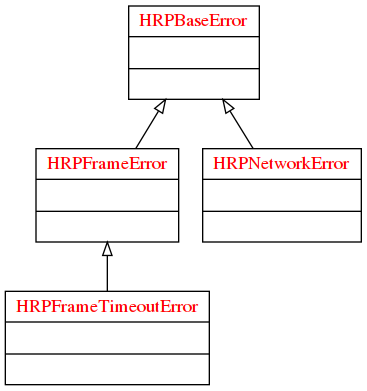
\includegraphics[width=0.6\linewidth]{classes_HRP_exception.png}
\newline Fuente: Elaboración propia
\label{fig:hrp_exception}
\end{figure}

\paragraph {util.py} contiene algunas funciones de bitácora, la función \_ord() para compatibilidad entre python2 y python3, y la función crc16(data), para el cálculo de la verificación de redundancia \footnote{actualmente la implementación sólo genera esta verificación para enviar datos al lector, aún no implementa una verificación de la integridad de la trama, ya que al utilizar TCP no es muy necesario}.

\paragraph{tag.py} define la clase Tag, y las clases para los parámetros de filtro o lectura de datos.

\begin{figure}[ht]
\caption{hrp.Tag}
\centering
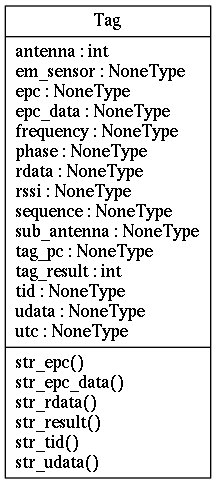
\includegraphics[width=0.35\linewidth]{classes_HRP_tag.png}
\newline Fuente: Elaboración propia
\label{fig:hrp_tag}
\end{figure}

Tiene como argumentos para la creación de un tag: la antena origen (\pythoninline{antenna}) y su RSSI (\pythoninline{rssi}), el EPC (\pythoninline{epc}), el PCW (\pythoninline{tag_pc}) y el resultado (\pythoninline{tag_result}) de la lectura, el resto de los argumentos son opcionales (\pythoninline{tid}, \pythoninline{udata}, \pythoninline{rdata}, \pythoninline{epc_data}, etc) y son poblados dependiendo el tipo de lectura que se realizó. Para la representación en texto (\pythoninline{str()}) dispone métodos de apoyo para cada tipo de argumento.  

\paragraph{hrp.py} define la clase HRP que se encarga de realizar todas las comunicaciones correspondientes con el lector

\begin{figure}[ht]
\caption{hrp.HRP}
\centering
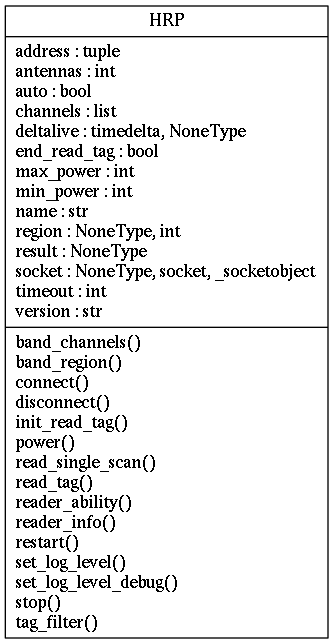
\includegraphics[width=0.6\linewidth]{classes_HRP_hrp.png}
\newline Fuente: Elaboración propia
\label{fig:hrp_hrp}
\end{figure}

la inicialización de la clase tiene como argumentos: la (\pythoninline{ip}) o host del lector, (\pythoninline{port}) o el puerto de comunicación (por defecto 9090), (\pythoninline{ommit_ping}) para omitir realizar un ping antes de iniciar a comunicación \footnote{Se agregó esta opción para permitir la implementación en contenedores que no posean el comando ping, o en S.O. que bloqueen el uso de este comando}, (\pythoninline{timeout}) que indica el tiempo de espera al realizar la comunicación TCP (por defecto  espera 10s antes de emitir un error de \pythoninline{HRPFrameTimeoutError}.

Para iniciar la comunicación con el lector se utiliza el método \pythoninline{connect()} el cual verifica la conexión ejecutando un ping, y luego crea el socket. A continuación, lee la información del lector \pythoninline{reader_info()} que puebla las propiedades de version, name y deltalive, con la versión del firmware, el nombre del lector y el tiempo de encendido del mismo. Luego obtiene la información de potencias \pythoninline{reader_ability()}, que puebla las propiedades de \pythoninline{min_power}, \pythoninline{max_power}, \pythoninline{antennas}, con las potencias mínimas y máximas soportadas, la máscara de antenas disponibles y retorna la lista de bandas y protocolos disponibles. Y luego obtiene la región actual con \pythoninline{band_region()} poblando a propiedad \pythoninline{region}, y los canales habilitados con \pythoninline{band_channels()} y poblando \pythoninline{channels}, lo cual permite verificar el uso correcto del ancho de banda y el espectro permitido en Bolivia. Finalmente lee la potencia actual de cada antena con el método \pythoninline{power()}.

Existe dos métodos para realizar la lectura de etiquetas, \pythoninline{read_single_scan()} y \pythoninline{read_tag()}, ambos métodos tienen los mismos argumentos, (\pythoninline{antenna}) para indicar la máscara de antenas \footnote{Donde cada bit corresponde a que antena estará habilitada para el escaneo}, (\pythoninline{match}) es un argumento del tipo \pythoninline{MatchParameter()} para indicar el filtro a aplicar en la lectura \footnote{ MatchParameter tiene tres argumentos (area, start, content) donde área es MATCH\_EPC o MATCH\_TID para indicar el área a aplicar el filtro, start es el bit de inicio para la comparación y content es el contenido en cadena de bytes a comparar, como limitante de la implementación, solo se pueden comparar bytes enteros}, el parámetro (\pythoninline{tid}) es un argumento del tipo \pythoninline{TidReadParameter()} que indica el tipo y tamaño de lectura del TID, los parámetros (\pythoninline{udata}, \pythoninline{rdata}, \pythoninline{edata}) son parámetros tipo \pythoninline{TagAddress()} que indican el inicio y el tamaño en palabras para leer las áreas de memoria de usuario, Reservado y EPC respectivamente \footnote{Permitiendo este parámetro edata, leer los datos adicionales del área EPC, que se utiliza para leer la información de los Tags SOAT}, en caso de requerirse, se puede dar el parámetro de (\pythoninline{password}) para indicar la contraseña de acceso.

La diferencia entre los métodos \pythoninline{read_single_scan()} y \pythoninline{read_tag()} es que \pythoninline{read_single_scan} realiza un solo barrido con la antena, y devuelve una lista \pythoninline{[Tag]} con todos las etiquetas que han sido detectadas, esta lista estará vacía si no se detectó ninguna etiqueta. el método \pythoninline{read_tag()} retorna un generador \footnote{Un tipo de función de Python, que permite devolver un resultado dinámicamente, para un consumo secuencial} que se utiliza para obtener interactívamente instancias de  \pythoninline{Tag} cuando son detectadas etiquetas, y \pythoninline{None} si no detecta ninguna  durante  \pythoninline{timeout}. Para finalizar el generador se debe colocar la propiedad  \pythoninline{end_read_tag} en  \pythoninline{True}\footnote{O generar una interrupción de teclado o finalizar el sistema}.

Para finalizar la comunicación con el lector se utiliza el método \pythoninline{disconnect()}, el cual permite detener cualquier lectura en espera, y cierra el socket TCP.

\subsection*{Ejemplos}

Se ha preparado tres ejemplos simples, que se encuentran en la carpeta \lstinline{examples/}. El ejemplo básico, utiliza el generador \pythoninline{read_tag()}

\begin{python}
from hrp import HRP, const, exception

try:
    conn = HRP('192.168.1.116', 9090)
    print ("Connectando")
    conn.connect()
    print ("presione Ctrl+C para terminar")

    counter = 0
    for tag in conn.read_tag(
            antennas=const.ANTENNA_1|const.ANTENNA_2):
        if tag is None:
            print ("Time out, {}".format(counter))
            counter += 1
            if counter > 10:
                conn.end_read_tag = True
        else:
            print (tag) #tag valido
except Exception as e:
    print ("Process terminate : {}".format(e))
finally:
    print ("Desconectando, bye!")
    conn.disconnect()
\end{python}

\subsection*{Filtrado de B-SISA y SOAT}

Luego de realizar pruebas se procedió a realizar lecturas esporádicas de vehículos en tránsito. posteriormente, la ANH confirmó la siguiente estructura del EPC de las etiquetas B-SISA

\begin{table}[hbt]
\caption{EPC del B-SISA}
\centering
\begin{tabular}{@{}ll@{}}
\toprule
Header    & 01 \\ 
Filter    & 01 \\ 
Partition & 98 \\ 
Company   & C00100 \\ 
Class     & XXXXXX \\ 
Serial    & YYYYYY \\ 
\bottomrule
\end{tabular}
\newline Fuente: \emph{ANH} 
\end{table}

la Clase corresponde al número de la etiqueta (codificado en mod10 para el código de barras) pero se puede notar que el inicio para el B-SISA siempre será 010198C00100.

Una forma simple de leer sólamente etiquetas de B-SISA es:

\begin{python}
import codecs
from hrp import HRP, const, exception
from hrp.tag import TidReadParameter, TagAddress
from hrp.tag import MatchParameter

BSISA_START = codecs.decode("010198C00100", "hex")
try:
    conn = HRP('192.168.1.116', 9090)
    print ("Connectando")
    conn.connect()
    print ("presione Ctrl+C para terminar")

    counter = 0
    for tag in conn.read_tag(
            antennas=const.ANTENNA_1|const.ANTENNA_2,
            match=MatchParameter(const.MATCH_EPC,
                                     0x20, BSISA_START),
            tid=TidReadParameter(0, 6)):
        if tag is None:
            print ("Time out, {}".format(counter))
            counter += 1
            if counter > 10:
                conn.end_read_tag = True
        else:
            print (tag) #tag valido
except Exception as e:
    print ("Process terminate : {}".format(e))
finally:
    print ("Desconectando, bye!")
    conn.disconnect()
\end{python}

En este caso, utilizamos el Filtro \pythoninline{MatchParameter} para indicar que sólo lea EPC empezando con la secuencia B-SISA, además de leer el TID de dicha etiqueta.

Para el caso del SOAT, las pruebas monstraron que el EPC que devuelve es único y corresponde a 00000000 00000024 00000000, esta etiqueta es un caso particular, puesto que el EPC reportado es de 96 bits, pero los datos que corresponden al código de barras se encuentran también en el área de memoria EPC, por lo que debemos leer datos adicionales de esa área.

\begin{python}
import codecs
from hrp import HRP, const, exception
from hrp.tag import TidReadParameter, TagAddress
from hrp.tag import MatchParameter

SOAT_START = codecs.decode("0000000000000024",
                               'hex')
try:
    conn = HRP('192.168.1.116', 9090)
    print ("Connectando")
    conn.connect()
    print ("presione Ctrl+C para terminar")

    counter = 0
    for tag in conn.read_tag(
            antennas=const.ANTENNA_1|const.ANTENNA_2,
            match=MatchParameter(const.MATCH_EPC,
                                     0x20, SOAT_START),
            tid=TidReadParameter(0, 6),
            edata=TagAddress(0x08, 2)):
        if tag is None:
            print ("Time out, {}".format(counter))
            counter += 1
            if counter > 10:
                conn.end_read_tag = True
        else:
            print (tag) #tag valido
except Exception as e:
    print ("Process terminate : {}".format(e))
finally:
    print ("Desconectando, bye!")
    conn.disconnect()
\end{python}

en este caso, el \pythoninline{Tag} leido tendrá un campo adicional \pythoninline{epc_data} con los 4 bytes que corresponden al código de barras de la etiqueta. al intentar leer campos adicionales del EPC\_data, impide la correcta lectura de B-SISA pudiéndose sólamente obtener el EPC del mismo\footnote{Ya que responde con un tag\_result=6 (Invalid data) y no devuelve el valor del TID}.

Si bien ambos tags sólo permiten su autoidentificación (corroborar la lectura con el código de baras) ninguno aprovecha el espacio de memoria de datos, para almacenar datos como ser la placa u otros datos del vehículo, el SOAT tiene planificado implementar dicha funcionalidad. para ello sólo se requerirá leer los campos de datos del tag:

\begin{python}
...
    for tag in conn.read_tag(
            antennas=const.ANTENNA_1|const.ANTENNA_2,
            match=MatchParameter(const.MATCH_EPC,
                                     0x20, SOAT_START),
            tid=TidReadParameter(0, 6),
            udata=TagAddress(0x28, 44),
            edata=TagAddress(0x08, 2)):
...
\end{python}

El campo de datos del SOAT tendrá dos espacios, un aŕea codificada que contendrá la placa y otros datos del vehículo, y otra área con datos como color, modelo y año del vehículo.
\begin{python}
...
            if tag.udata:
                #quitar espacios
                data = str(tag.udata).strip()
                #dvidir espacio codificado
                cdata = data.split('|')
                pdata = base64.b64decode(cdata[0])
                #placa vehiculo
                placa = pdata.split('>')[0]
...
\end{python}

Si bien el despliegue de dichos campos aún no está en el parque automotor\footnote{Sólo en las etiquetas de prueba provistas por Quipus}.

\subsection*{Lectura de B-SISA y SOAT}

Para leer ambos tipos de etiquetas al mismo tiempo, se optó por una lectura más secuencial, leyendo cualquiert tag, y forzando una segunda lectura en caso de encontrar un SOAT.

\begin{python}
import codecs
from hrp import HRP, const, exception
from hrp.tag import TidReadParameter, TagAddress
from hrp.tag import MatchParameter

BSISA_START = codecs.decode("010198C00100", "hex")
SOAT_START = codecs.decode("0000000000000024",
                               'hex')
try:
    conn = HRP('192.168.1.116', 9090)
    print ("Connectando")
    conn.connect()
    print ("presione Ctrl+C para terminar")

    counter = 0
    while True:
        tags = conn.read_single_scan(
            antennas=const.ANTENNA_1|const.ANTENNA_2,
            tid=TidReadParameter(0, 6)):
        if not tags:
            print ("Time out, {}".format(counter))
            continue
        for tag in tags:
            if tag.epc[:len(SOAT_START)] == SOAT_START:
                soat = conn.read_single_scan(
                    antennas=const.ANTENNA_1 |
                               const.ANTENNA_2,
                    match=MatchParameter(
                                   const.MATCH_TID,
                                   0x0, tag.tid),
                    tid=TidReadParameter(0, 6),
                    edata=TagAddress(0x08, 2))
                if soat and soat[0].tag_result == 0:
                    tag = soat[0] # remplazar
            print (tag) #tag valido
except Exception as e:
    print ("Process terminate : {}".format(e))
finally:
    print ("Desconectando, bye!")
    conn.disconnect()
\end{python}

\subsection*{Pruebas de Campo}

para facilitar las pruebas de campo se desarrolló una aplicación web mediante FLASK y SOCKET.IO generando una pequeña interfaz web y generando un websocket cada vez que se detecta un tag válido, mostrándose en tiempo real en la interfaz web. También se aprovechó para almacenar los datos registrados en una base de datos PostgresQL

\begin{figure}[ht]
\caption{Captura Tags}
\centering
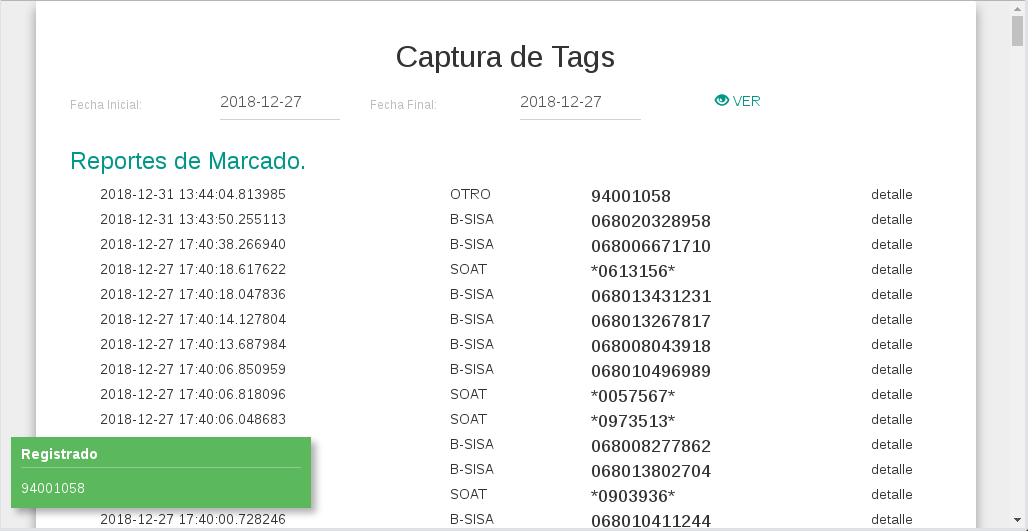
\includegraphics[width=\linewidth]{captura_lector}
\newline Fuente: Elaboración Propia
\label{fig:captura_tag}
\end{figure}

\begin{figure}[ht]
\caption{Captura Tags: Detalle}
\centering
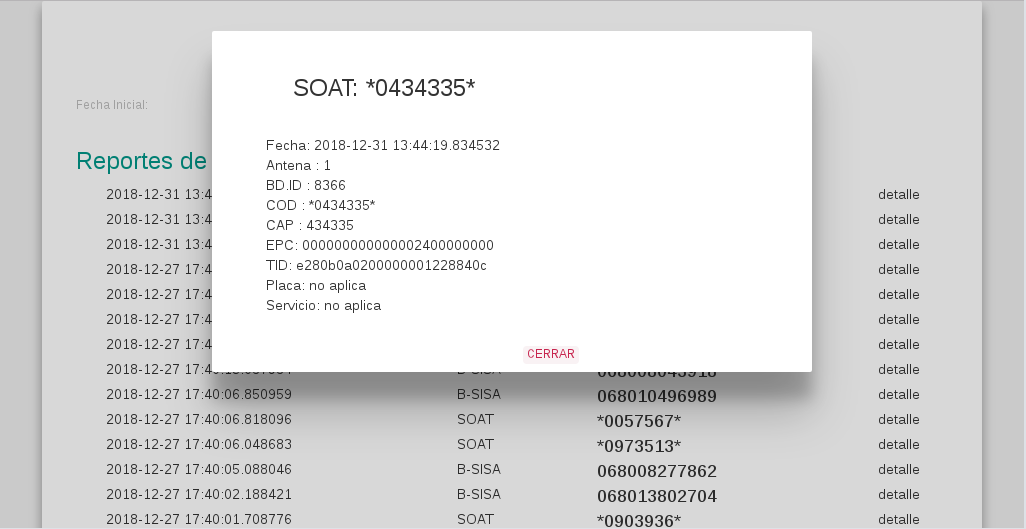
\includegraphics[width=\linewidth]{captura_detalles}
\newline Fuente: Elaboración Propia
\label{fig:captura_detalles}
\end{figure}

\section{Resultados}

Con el sistema funcionando, se realizó un par de pruebas: La primera en la calle Ecuador esquina Pedro Salazar, registrando los vehículos de subida y comparando con una grabación de los vehículos para ver la ubicación de las etiquetas.

de 102 vehículos que circularon en un lapso de 15 minutos, sólo se indentificó 57 lecturas de SOAT (56\%) y 72 lecturas de B-SISA (70\%)


Para el análisis de datos, se optó por alimentar la información de las antenas a un red ADS-B con mayores prestaciones. obtándose por la red OpenSkyNetwork, que ofrece herramientas estadísticas sobre el rendimiento de los receptores.

\subsection*{El Alto}

El primer receptor instalado, tiene un buen desempeño\footnote{https://opensky-network.org/receiver-profile?s=-1408236454} con un rango entre 180 a 300 km cubriendo un área de 35.000 a 62.000 km2, con un promedio de 550 mensajes procesados por dia (llegando a 44 mensajes por segundo) y capturando hasta 50 aeronaves por día.

\begin{figure}[ht]
\caption{El Alto: Rango de 1 día}
\centering
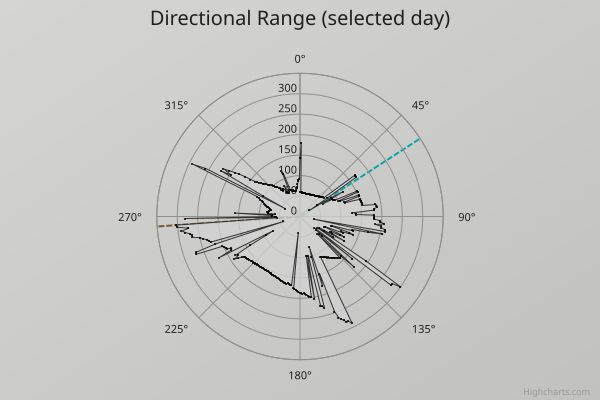
\includegraphics[width=0.8\linewidth]{lpb_range.png}
\newline Fuente: OpenSky Network
\label{fig:lpb_range}
\end{figure}

\begin{figure}[ht]
\caption{El Alto: Disponibilidad}
\centering
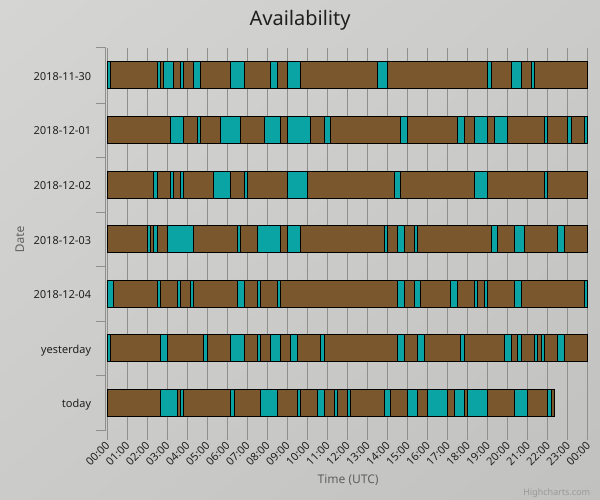
\includegraphics[width=0.8\linewidth]{lpb_disp.png}
\newline Fuente: OpenSky Network
\label{fig:lpb_disp}
\end{figure}

\begin{figure}[ht]
\caption{El Alto: Promedio de mensajes}
\centering
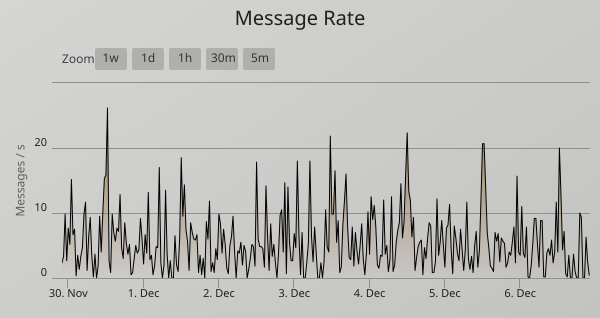
\includegraphics[width=0.8\linewidth]{lpb_mes.png}
\newline Fuente: OpenSky Network
\label{fig:lpb_mes}
\end{figure}

\subsection*{Cochabamba}

Pese a ser un mejor receptor, esta antena tuvo un rendimiento medio\footnote{https://opensky-network.org/receiver-profile?s=-1408236489}, recalcando de esta forma la importancia de la ubicación y la línea de vista \footnote{Recordemos que cochabamba es un valle rodeado de cerranías}. Tiene un rango entre 150 a 220km, cubriendo un área entre 25.000 a 40.000 km2, con 450.000 mensajes procesados por día (llegando a 32 mensajes por segundo) y capturando hasta 60 aeronaves por día.

\begin{figure}[ht]
\caption{Cochabamba: Rango de 1 día}
\centering
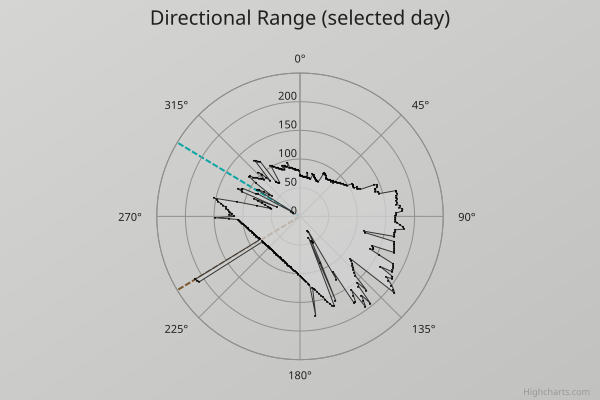
\includegraphics[width=0.8\linewidth]{cbb_range.png}
\newline Fuente: OpenSky Network
\label{fig:cbb_range}
\end{figure}

\begin{figure}[ht]
\caption{Cochabamba: Disponibilidad}
\centering
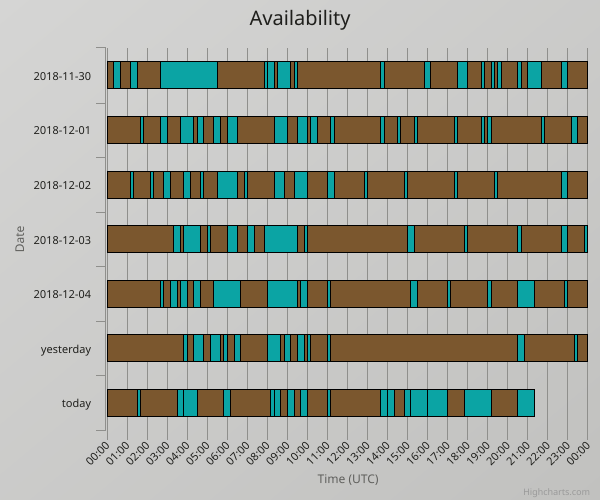
\includegraphics[width=0.8\linewidth]{cbb_disp.png}
\newline Fuente: OpenSky Network
\label{fig:cbb_disp}
\end{figure}

\begin{figure}[ht]
\caption{Cochabamba: Promedio de mensajes}
\centering
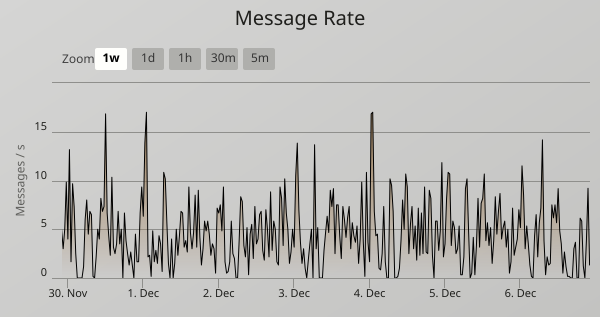
\includegraphics[width=0.8\linewidth]{cbb_mes.png}
\newline Fuente: OpenSky Network
\label{fig:cbb_mes}
\end{figure}


\subsection*{Santa Cruz}

Esta fue la antena con el mejor rendimiento\footnote{https://opensky-network.org/receiver-profile?s=-1408236530}, con un promedio de 500km de rango direccional, cubriendo un área entre 200.000 a 350.000 km2, con 1.250.000 mensajes procesados por día (llegando a 32 mensajes por segundo) y capturando hasta 100 aeronaves por día.

\begin{figure}[ht]
\caption{Viru Viru: Rango de 1 día}
\centering
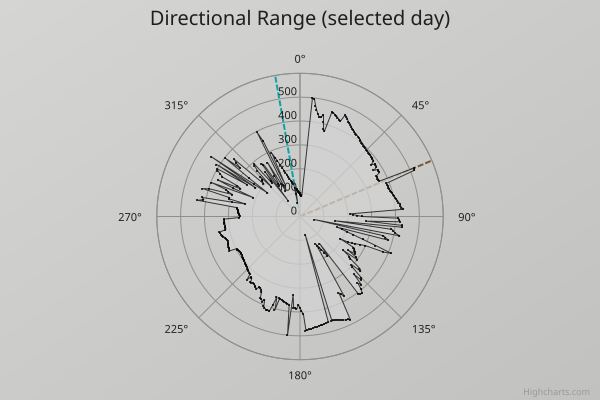
\includegraphics[width=0.8\linewidth]{vvi_range.png}
\newline Fuente: OpenSky Network
\label{fig:vvi_range}
\end{figure}

\begin{figure}[ht]
\caption{Viru Viru: Disponibilidad}
\centering
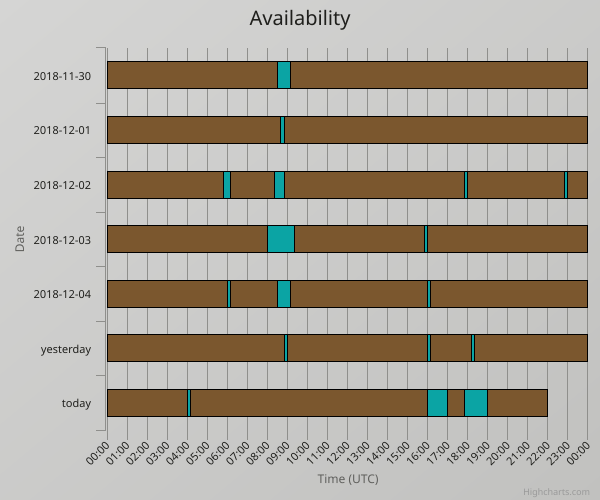
\includegraphics[width=0.8\linewidth]{vvi_disp.png}
\newline Fuente: OpenSky Network
\label{fig:vvi_disp}
\end{figure}

\begin{figure}[ht]
\caption{Viru Viru: Promedio de mensajes}
\centering
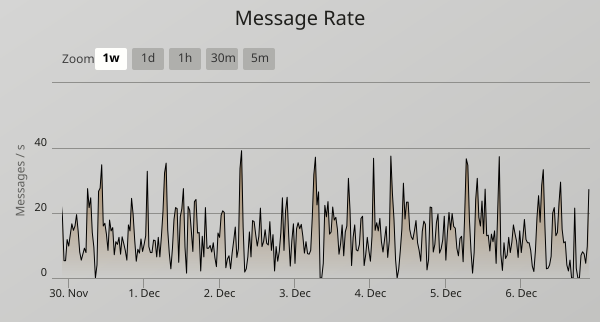
\includegraphics[width=0.8\linewidth]{vvi_mes.png}
\newline Fuente: OpenSky Network
\label{fig:vvi_mes}
\end{figure}

\section{Conclusiones}

Tan sólo colocando 3 antenas receptoras ADS-B se ha logrado cubrir un 50\% del territorio boliviano. Aunque se pudo evidenciar que la mayoría de las aeronaves nacionales (principalmente de la línea amaszonas) solo envían mensajes en Modo-S, impidiendo obtener su ubicación con el arreglo actual. Para ello, se puede utilizar una técnica llamada multilateración MLAT, que con 3 o más receptores ADS-B separados espacialmente en 5km o más \footnote{Es decir en un arreglo cuadrático o circular, evitando formar una sola línea de sensores}.

También se evidenció pequeñas falencias en los transpondedores de algunas aeronaves nacionales, que tienen bastante interferencia (posiblemente por falta de calibración en el mismo transpondendor) e incluso varias aeronaves que tiene un arrastre de la señal GPS por falta de calibración en sus antenas.

Si se implementara un sistema de recepción ADS-B que no entre en conflicto con el SIVICEA (o incluso que pueda trabajar en conjunto para corroborar - certificar la información) se debería ver de instalar más antenas en nuestro territorio.

%----------------------------------------------------------------------------------------
%	REFERENCE LIST
%----------------------------------------------------------------------------------------
\phantomsection
\bibliographystyle{unsrt}
\bibliography{bibliografia}{}

%----------------------------------------------------------------------------------------

\end{document}
